% !TEX root = main.tex
\chapter{A New Uni-Authoritative Paradigm for Certificate Issuance}

% ==============Introductory Remarks====================== %
\section{Introductory Remarks}
\label{sec:chap4Introductory Remarks}

%===================================================%
\begin{figure}[t]
\centering
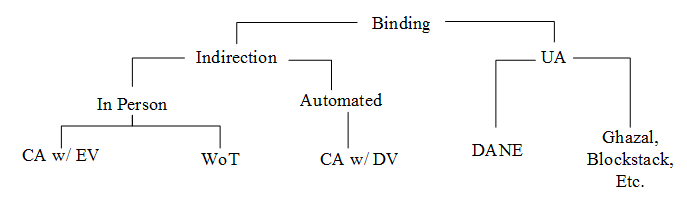
\includegraphics[width=0.9\textwidth]{Fig/binding.png}
\caption{\footnotesize{Different approaches to provide the binding between a namespace and cryptographic public keys.}}
\label{fig:Binding}
\end{figure}
%===================================================%

In the previous chapter we discussed domain control verification (DCV) techniques and the primary issues with these procedures. Our findings were largely based upon our empirical study that investigates how the certificate authorities actually issue certificates to the end users and how they verify the ownership of domain names. Actual failures in domain validation procedures occur when CAs are not effectively successful in verifying the subjects identities, therefore, enabling the registration of a public key under another entity's already-registered domain name.

Issuing certificates is equal to binding names from a namespace to cryptographic keys. To provide this binding, a system can either rely on indirection and have certificate authorities that are not authoritative over the namespace try to verify ownership; or it can collapse the indirection if the issuing entity is authoritative over the namespace---we call this the \UA paradigm (see Figure~\ref{fig:Binding}). In the current web certification model, CAs heavily rely on indirection to verify the ownership of the namespace and provide the binding. Technically, they can validate the namespace ownership via (i) DCV methods which are typically automated and effortless and/or (ii) in-person validation techniques. In-person includes high assurance certificates (EV,OV) which are validated by the CA using government-issued documents, or Web-of-Trust (WoT) where external parties validate and sign off on one's identity typically also after checking some government-issued ID. Note that in-person validation is still indirection as the government is authoritative over its citizen's names or registered business names, while CAs are typically non-government entities (and even when CAs are governmental, they are authoritative over all domains including ones not owned by their citizens). From here forward, we consider the case of automated domain validated certificates. 

In the \UA paradigm, the owner of the namespace is fully authoritative over it and is the same entity that binds names to cryptographic keys. In this thesis, we explore this in the context of blockchain technology. If a PKI were added to a blockchain, who would be authoritative over the namespace of domain names? When domain names themselves are issued through the blockchain (\eg Namecoin), then the blockchain is actually the authoritative entity. Such a design would thus be \UA. 

Arguably, indirection can be collapsed in the traditional web certificate model as well. As we argued in the previous chapter, DNS (in conjunction with ICANN) is authoritative over the namespace of domain names. If ICANN/DNS held key bindings, there would be no indirection or CAs needed. Indeed exactly this has been proposed under the same of DNS-based Authentication of Named Entities (DANE). Thus blockchains and DANE are both examples of a \UA paradigm. A deployment issue with DANE is that DNS records do not generally have message integrity (except via the under-deployed DNSSEC) whereas blockchain transactions do. 

As it was mentioned in the previous chapter, a variety of attacks in the current CA ecosystem show these third parties' inability to provide an authentic and proper binding between the namespaces and the cryptographic keys --- where adversaries were able to acquire fraudulent certificates for domains they do not control. incorrect bindings can be either (i) prevented or (ii) detected.  As it can be seen in Figure ~\ref{fig:prevention}, prevention techniques can be applied by any CAs and/or any sites to prevent from a wrong binding. For example, a domain owner could add a CAA record to his DNS where he declares a list of CAs that are allowed to issue a certificate for his domain (IKP is a blockchain analogue); he could hardcode his certificate or constraints on his certificate into the browser the user will install (\eg key pins in Google Chrome); or he could pin his certificate the first time the user visits his site to protect subsequent visits (TACK) assuming the first interaction is trustworthy (trust-on-first-use or TOFU). 

%===================================================%
\begin{figure}[t]
\centering
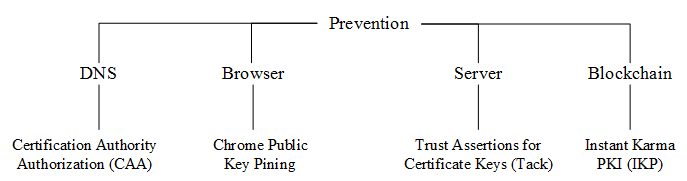
\includegraphics[width=0.9\textwidth]{Fig/prevention.png}
\caption{\footnotesize{Techniques to prevent from incorrect (namespace, keys) bindings.}}
\label{fig:prevention}
\end{figure}

%===================================================%

%===================================================%
\begin{figure}[t]
\centering
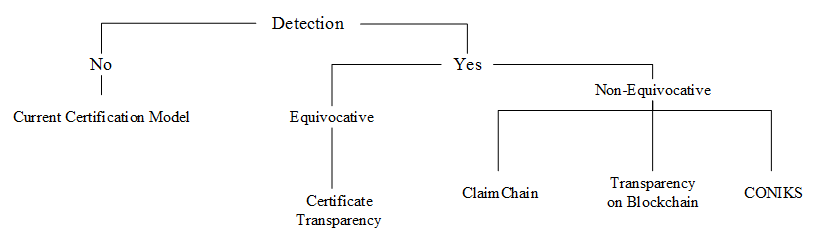
\includegraphics[width=0.9\textwidth]{Fig/detection2.png}
\caption{\footnotesize{Techniques to add visibility about (namespace, keys) bindings.}}
\label{fig:detection}
\end{figure}
%===================================================%

Unlike prevention techniques, detection methods do not prevent wrong bindings from occurring, instead they add visibility and transparency about (namespace, keys) binding, so it can be detected in case of failures. In the traditional web certification model, CAs do not provide any insight about this binding. Lack of the visibility of bindings has led to several failures; thus, attempts have been made to add transparency to the CAs ecosystem (see Figure ~\ref{fig:detection} ). Certificate transparency (CT)~\cite{laurie2014certificate}, sovereign keys (SKs) \cite{giteffor4:online}, and ARPKI \cite{basin2014arpki} are systems that augment the current web certificate mode by supplying a log of CA-issued certificates. A step further is not to rely on CAs at all; another group of transparency solutions rely on users validating their own entry in the log and then enforcing that all users see the same entry when referencing the log even if the server hosting the log is malicious (a property called non-equivocation). CONIKS is such a system and provides a distributed log but for public keys \cite{melara2015coniks}. ClaimChain is similar to CONIKS but finds a middle-ground between using a small set of distributed servers (CONIKS) and a fully decentralized but global state (blockchain) by having fully decentralized, local states that can be cross-validated \cite{kulynych2017claimchain}.

\section{The \Ghazalstar System}

Our proposed scheme is entitled \Ghazalstar, a smart contract-based naming and PKI \UA system. \footnote{\GhazalCode} \Ghazalstar is is actually a new \UA paradigm that resolves some of the fundamental issues with the current certification model --- authority and indirection. It enables entities, whether they are people or organizations, to fully manage and maintain control of their domain name without relying on trusted third parties. By proposing \Ghazalstar, we argue that adding programmability to a dapp-based PKI provides benefits beyond using the blockchain as an append-only broadcast channel.

Using our system, users can register unclaimed domain names as globally readable identifiers on the Ethereum blockchain, bind the domain name to arbitrary data \ie public keys \etc These values are globally readable, non-equivocating, and not vulnerable to the indirection attacks outlined in \autoref{chap:Understanding domain validation practices}. Anyone can claim a domain on a first-come, first-serve basis. Because it is decentralized, names cannot be re-assigned without the cooperation of the owner (whereas an ICANN address like \texttt{davidduchovny.com} can be re-assigned through adminstrative mediation). Another feature of \Ghazalstar system is speeding up the DNS updates. In our system, DNS resource records are updated in 12 seconds (block interval in the Ethereum blockchain), whereas it would take 3 days for users to update domain names resource records using the traditional DNS system.

This novel system consists of two essential elements. First, the smart contract that resides on the Ethereum blockchain and serves as the interface between entities and the underlying blockchain. The second primary component of the system are the clients, including people or organizations that interact with \Ghazalstar smart contract in order to manage their domain names. Figure ~\ref{fig:StateDiagram} represents the primary states a domain name can be in and how state transitions work. These states are enforced within the code itself to help mitigate software security issues related to unintended execution paths. 

% ==============State Diagram Figure====================== %
\begin{figure}[htb!p]
\centering
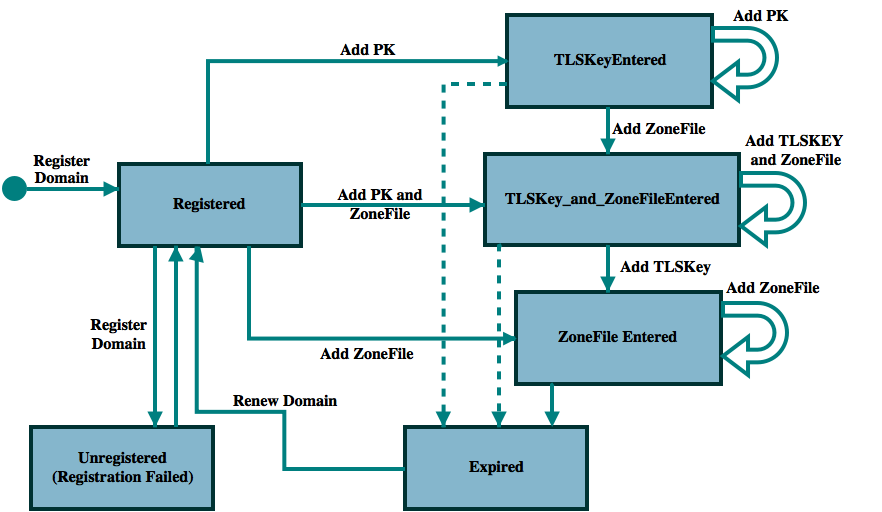
\includegraphics[width=0.9\textwidth]{Fig/StateDiagram-2.png}
\caption{\footnotesize{Primary states and transitions for a domain name in \Ghazalstar.}}
\label{fig:StateDiagram}
\end{figure}
%===================================================%

\subsection{Exploring \Ghazalstar design choices}

Beyond simply presenting our design, we think it is useful to explore the landscape of possible designs. To this end, we discuss some deployment issues that we faced where there was no obvious ``one right answer.'' These are likely to be faced by others working in this space (whether working narrowly on PKI or broad identity on blockchain solutions). 

% ==============Design Decision \#1: Domain Name Expiration================= %
\subsubsection[Domain Name Expiration]{Design Decision \#1: Domain Name Expiration}

Typically domain name ownership eventually \textit{expires}. Once a domain expires, it is returned to the primary market, except if the users renews it. However, expiration does not necessarily have to mean a disclaimer of ownership; there are other options. 
\begin{enumerate}

\item \textbf{Domain names never expire and last forever.} Designing a system with no domain name expiration would be highly vulnerable to domain squatting. Domain squatting is registering domain names in speculation that the will increase in value. These domain names generally do not point to any relevant IP address (except to earn revenue on accidental visits). If domain names never expire, squatting may be significantly problematic as squatted names would be locked forever while legitimate users will end up choosing unusual names from the remaining namespace. To be clear, even without expiration, if domains are cheap, squatting is problematic (\eg Namecoin~\cite{Kalodner2015empirical}). 

\item \textbf{Domain names get deleted once they expire, except being renewed by the user.} The most restrictive system design is where a domain name effectively gets deleted and is returned to the registry of unclaimed names once it expires, unless the user renews it. This model has the following two issues. First, if a browser tries to resolve an expired domain, because the blockchain has a complete, immutable history of that domain, we would expect users to want it resolved according to the previous owner. Rolling back expiration is possible in a way not supported by DNS and it resolves simple human errors of forgetting to renew domains, so we do not expect browsers to necessarily fail when it could make a sensible guess as to which server their users are looking for. The second reason to drop the deletion model of expiration is that Ethereum contracts can only run when a function is called. If no one calls a function at expiration time, the contract cannot self-execute to modify itself. The fact that it is expired can be inferred from contract if it includes a time but the contract itself will not transition states until someone calls a function that touches that particular contract. An alternative is to rely on a third party like Ethereum Alarm Clock~\cite{Home41:online} for scheduling future function calls. This is suitable only if the threat model permits relying on a trusted third party and a single point of failure (for this one feature). 

\item \textbf{Control over domain names is lost once they expire, except being renewed by user.} In \Ghazalstar, expired domains continue to function although the owner (i) looses the sole claim to that domain and cannot preserve it if someone else purchases it, and (ii) she cannot modify the domain in anyway (\eg add certificates or change zone information) unless if she first renews it. Essentially, purchasing a domain name does not entitle an entity to own it forever; expired domain names are returned back to the primary market and are available for all the users within the system. However since a full history of a domain is present, the system's best effort at resolving the domain will be to preserve the last known state. Expiration in conjunction to the amount of the fee will influence the degree of domain squatting, and having expiration at all will allow abandoned domains to churn if they are under demand. 

\end {enumerate}
% ==============Design Decision \#1b: Fees================= %
\subsubsection[Registration Fees]{Design Decision \#2: Registration Fees}

In \Ghazalstar, new registrations and renewals require a fee. This fee is a deterrent against domain squatting. The fee amount is difficult to set and no fee will be perfectly priced to be exactly too high for squatters but low enough for all `legitimate' users. Rather it will trade-off the number of squatters with the number of would-be legitimate users who cannot pay the fee. Namecoin is evidently too cheap and ICANN rates seem reasonable. We leave this as a free parameter of the system. The important decisions are: (1) in what currency are they paid and (2) to whom. Every Ethereum-based system, even without a fee, will at least require gas costs. Additional fees could be paid in Ether or in some system-specific token. Since it is a decentralized system and the fee is not subsidizing the efforts of any entity involved, there is no one in particular to pay. The fee could be paid to an arbitrary entity (the system designer or a charity), burned (made unrecoverable), or to the miners. In \Ghazalstar, fees are paid in Ether and are released to the miner that includes the transaction in the blockchain. 

% ==============Design Decision \#3: Domain Name Renewal====================== %
\subsubsection[Domain Name Renewal]{Design Decision \#3: Domain Name Renewal}

We design \Ghazalstar in such a way that the domain owners can renew their domains before their validity period comes to an end, however they cannot renew an arbitrary number of times. Specifically, a renewal period becomes active after the domain is past 3/4 of its validity period. Renewal pushes the expiration time forward by one addition of the validity period (thus renewing at the start or end of the renewal period is inconsequential and results in the domain having the same expiration time). Requiring renewal keeps users returning regularly to maintain domains, and unused domains naturally churn within the system. Domain name redemption period can take different values. We experiment with a validity period of 1 year; thus, the renewal period would start after 9 months and last 3 months. 

% ==============Design Decision \#4: Domain Name Ownership Transfer====================== %
\subsubsection[Ownership Transfer]{Design Decision \#4: Domain Name Ownership Transfer}
\label{sec:revocation}

\begin{lstlisting}[basicstyle=\scriptsize\ttfamily,caption={Implementation of AuctionStruct and AuctionLists mapping in \Ghazalstar smart contract.},label={code:auction},float]
//Possible states of every auction.
enum <@\textcolor{cyan}{Stages}@> {Opened, Locked, Ended} 
   
    struct AuctionStruct  
    {  uint CreationTime;  
        address Owner;    
        uint highestBid;    
        address highestBidder;  
        address Winner;   
        Stages stage;           
        //To return the bids that were overbid.
        mapping(address => uint) pendingReturns;   
	      //To return the deposits the bidders made. 
        mapping(address => uint) deposits;      
        //Once an address bids in the auction, its associated boolean value will be set to true within the "already_bid" mapping.
        mapping(address => bool) already_bid;      
        bool AuctionisValue;                        
      }
//AuctionLists mappings store AuctionStructs.
mapping (bytes32 => AuctionStruct) internal AuctionLists;
\end{lstlisting}

\noindent In \Ghazalstar, domain owners can transfer the ownership of their unexpired domains to new entities within the system. Basically, transferring a domain name at the Ethereum level means changing the address of the Ethereum account that controls the domain. Our system offers two ways of transferring the ownership of a domain:

\begin{enumerate}

\item \textbf{Auctioning off the domain name.} A domain owner can voluntarily auction off an unexpired domain. Once an auction is over, the domain is transferred to the highest bidder, the payment goes to the previous owner of the domain, and the validity period is unaffected by the transfer (to prevent people from shortcutting renewal fees by selling to themselves for less than the fee). If there are no bidders or if the bids do not reach a reserve value, the domain is returned to the original owner. While under auction, a domain can be modified as normal but transfers and auctions are not permitted. To implement the auction feature, we use the fact that Solidity is object-oriented. We first deploy a basic \Ghazal function without advanced features like auctions, and then use \textit{inheritance} to create a child contract \Ghazalstar that adds the auction process. Using \Ghazalstar, a user can run any number of auctions on any number of domains he owns. This is implemented through a mapping data structure called \textit{AuctionLists} to store every auctions along with its attributes. \textit{AuctionLists} accepts \textit{Domain names} as its keys, and the \textit{AuctionStructs} as the values (see Code~\ref{code:auction}). Using the mapping and Ethereum state machine, we enforce rules to prevent malicious behaviors \eg domain owners can auction off a domain only if there is no other auction running on the same domain. To encourage winners to pay, all bidders must deposit a bounty in Ether the first time they bid in an auction (amount set by the seller). This is refunded to the losers after bidding closes, and to the winner after paying for the domain. Without this, users might disrupt an auction by submitting high bids with no intention of paying. 


\begin{lstlisting}[basicstyle=\scriptsize\ttfamily,caption={\texttt{Transfer\_Domain} function of  \Ghazalstar smart contract.}, label={code:transfer}]
modifier CheckDomainExpiry(bytes32 _DomainName) {
       if (Domains[_DomainName].isValue == false) 
          {Domains[_DomainName].state=States.Unregistered;} 
       if (now>=Domains[_DomainName].RegistrationTime+10 minutes)
          {Domains[_DomainName].state = States.Expired;} 
        _;
    }
modifier Not_AtStage(bytes32 _DomainName, States stage_1, States stage_2) {
        require (Domains[_DomainName].state != stage_1 && Domains[_DomainName].state != stage_2);
        _;
    }
modifier OnlyOwner(bytes32 _DomainName) {
        require(Domains[_DomainName].DomainOwner == msg.sender);
        _;
    }        
function Transfer_Domain(string _DomainName,address _Reciever,bytes32 _TLSKey, string _IP_Adress) public 
CheckDomainExpiry(stringToBytes32(_DomainName)) 
Not_AtStage(stringToBytes32(_DomainName),States.Unregistered,States.Expired) 
OnlyOwner(stringToBytes32(_DomainName))
    {
        DomainName = stringToBytes32(_DomainName);
        Domains[DomainName].DomainOwner = _Reciever;
        if (_TLSKey == 0 && stringToBytes32(_IP_Address) != 0) { Wipe_TLSKeys(DomainName); }
        if (stringToBytes32(_IP_Address) == 0 && _TLSKey != 0 ) {  Wipe_IP_address(DomainName); }
        if (stringToBytes32(_IP_Address) == 0 && _TLSKey == 0 ) { Wipe_TLSKeys_and_IP_address(DomainName); }
    }
\end{lstlisting}

\item \textbf{Transfer the ownership of a domain name.} A domain owner can also transfer an unexpired domain to the new Ethereum account by calling the \textit{Transfer\_Domain} function which simply changes the Ethereum address that controls the domain name. The owners can also decide to either transfer domain's associated attributes (\eg TLS certificates) or not, when they transfer the domain. This is possible with either supplying these attributes with zero or other desired values when calling the \texttt{Transfer\_Domain} function (see Code~\ref{code:transfer}).

\end{enumerate}

To prevent from MITM attacks, TLS certificates should be revoked once a domain name is transferred. However, security incidents reveal that this is not commonly enforced in the current PKI. For instance, Facebook acquired the domain \texttt{fb.com} for \$8.5M in 2010, yet no one can be assured if that the previous owner does not have a valid unexpired certificate bound to this domain~\cite{CO13}. This has been successfully enforced in our system as the new owner of the domain is capable of modifying the domain's associated TLS keys, which results in protecting communications between the clients and his server from eavesdropping.

% =======Design Decision \#6: SPV Friendly Certificate Revocation====================== %
\subsubsection[Toward Lightweight Certificate Revocation]{Design Decision \#5: Toward Lightweight Certificate Revocation}\label{LESservers}

In the broader PKI literature, there are four traditional approaches to revocation \cite{myers1998revocatoin}: certificate revocation lists, online certificate status checking, trusted directories, and short-lived certificates. Revocation in the web certificate model is not effective. It was built initially with revocation lists and status checking, but the difficulty of routinely obtaining lists and the frequent unavailability of responders led to browsers failing open when revocation could not be checked. Some browsers build in revocation lists, but are limited in scope; EV certificates have stricter requirements; and some research has suggested deploying short-lived certificates (\eg four days) that requires the certificate holders to frequently renew them~\cite{topalovic2012towards} (in this case, certificates are not explicitly revoked, they are just not renewed). Which model does a blockchain implement? At first glance, most blockchain implementations would implement a trusted directory: that is, a public key binding is valid as long as it is present and revocation simply removes it. The issue with this approach on a blockchain is how users establish they have the most recent state. With the most recent state in hand, revocation status can be checked. This check is potentially more efficient than downloading the entire blockchain (this functionality exists for Bitcoin where it is called SPV and is a work in progress for Ethereum where it is called LES). However a malicious LES server can always forward the state immediately preceding a revocation action and the client cannot easily validate it is being deceived.

At a foundational level, most revocation uses a \texttt{permit-override} approach where the default state is permissive and an explicit action (revocation) is required. Short-lived certificates (and a closely related approach of stapling a CA-signed certificate status to a certificate) are \texttt{deny-override} meaning the default position is to assume a certificate is revoked unless if there is positive proof it is not. This latter approach is better for lightweight blockchain clients as LES servers can always lie through omitting data, but cannot lie by including fraudulent data (without expending considerable computational work). As an alternative or compliment, clients could also take the consensus of several LES servers, although this `multi-path probing' approach has some performance penalties (it has been suggested within the web certificate model as Perspectives~\cite{WAP08} and Convergence~\cite{Mar11}). 

In \Ghazalstar, public keys that are added to a domain name expire after a maximum lifetime, \eg four days. Expiration is not an explicit change of state but is inferred from the most recent renewal time. Owners need to rerun the key binding function every several days to renew this. If an owner wants to revoke a key, she simply fails to renew. To verify the validity of a certificate, one is now able to use a LES-esque protocol. Once a user queries a semi-trusted LES node for a corresponding record of a domain, the node can either return a public key that is four days old, which user will assume is revoked, or a record that newer that the user will assume is not revoked. Although this approach requires the frequent renewal of public keys, it is a cost that scales in the number of domains as opposed to revocation checks which scale in the number of users accesses a domain. 

% ==============Ghazal OPerations (Functions)====================== %
\section{\Ghazal Main Operations}
At the time of writing this thesis, there are 19 functions in \Ghazalstar (\Ghazal's child contract that adds the auction process). In this section, we represent a list of primary functions that are mainly used to mange (\eg register, renew, \etc) the domain names within our system.

% ==============Domain Registration====================== %
\paragraph{Domain Name Registration.}

\emph{Register} function allows entities to register unregistered or expired domain names.This function is \emph{payable} that is, entities need to pay the domain registration fees to call this function and claim the domain names. \emph{Register} function takes one parameter as its input; \textbf{Domain name}-- A string representing a domain name the user aims to claim.
% ==============Domain Renewal====================== %
\paragraph{Domain Name Renewal.}

\emph{Renew} function allows entities to renew their domain names before their validity period comes to an end.This function is \emph{payable} and takes one parameter as its input; \textbf{Domain name}-- A string representing a domain name the owner wants to renew.
% ==============Adding the TLS Key====================== %
\paragraph{Add Certificate.}

\emph{Add TLSKey} function allows domain name owner to bind TLS keys to his domain name. This function can be also used to overwrite the existing TLS keys in case of the private key loss or interception. It takes the followings as input: \par
\textbf{Domain name}-- A string representing a domain name to which the owner aims to bind the TLS keys. \par
\textbf{TLS Key}-- A dynamically sized byte array that stores TLS keys.

% ==============Adding the Add\_Zonefile====================== %
\paragraph{Add Zonefile.}
 
Using the \emph{Add Zonefile} function, domain owner can add the associated resource records to his domain name. Followings represent the input parameters of this function: \par
\textbf{Domain Name.} A string representing a domain name to which the owner aims to the resource records. \par
\textbf{IP Address.} An string representing the domain name's associated IP address.

% ==============Adding the TLS Key and DNS Hash====================== %
\paragraph{Add Certificate \& Zonefile.}

\emph{Add TLSKey \& Zonefile} function allows domain owners to bind TLS keys and zone files to their domain names simultaneously. This function takes the three following input parameters: \par
\textbf{Domain Name.} A string representing a domain name to which the owner aims to add the attributes.\par
\textbf{IP Address.} A string representing the domain name's associated IP address.\par
\textbf{TLS Key.} A dynamically sized byte array that stores TLS keys.

% ==============Revoke certificate====================== %
\paragraph{Revoke Certificates.}

\emph{Revoke Certificate} function allows domain owners to delete any specific certificate that is bound to their domains. This function takes two input parameters: \par
\textbf{Domain Name.} A string representing a domain name. \par
\textbf{TLS Key.} A dynamically sized byte array representing the TLS key that owner wants to revoke.
%===================================================%

\section{Walkthrough of Domain Name Resolution in \Ghazalstar}

This section provides a walkthrough of resolving a domain using the \Ghazalstar system.


\subsection{\Ghazalstar with \texttt{.ghazal} namespace}

In order to visit \texttt{bank.ghazal} website over HTTPS, the user's browser needs to resolve the IP address for \texttt{bank.ghazal} and obtain its public key. The browser might be configured in one of two ways to resolve domains---one method is more secure but has deployability challenges, while the other makes a trust assumption and gains efficiency. The first option is for the user's client to maintain a local copy of the Ethereum blockchain. In this case, the browser can query its local copy of the blockchain and parse the mapping data structure to recover the domain name's associated attributes (\eg DNS resource records and TLS certificates). Due to the data structure, accessing these values is performed in constant time because the mapping works like a hash table (so the entire list of domains does not have to be searched, as would be the case with an array---see Section~\ref{MapvsArray}). Additionally, because the blockchain is local, this introduces no extra rounds of communication (other than having the blockchain updated). This approach is the most secure way of resolving \texttt{.ghazal} domain names as the clients directly consult with the blockchain without relying on any other party. However, it requires clients to download and maintain the entire Ethereum blockchain, which is not feasible for lightweight blockchain clients such as smartphones. Another way of resolving the \texttt{bank.ghazal} domain name is to rely on semi-trusted full node LES servers. In this approach, instead of downloading the entire Ethereum blockchain, browsers can connect to LES severs and obtain the domains attributes. This check is more efficient than downloading the entire blockchain, however it is less secure as trust is involves trusting other parties who can be malicious. See Section~\ref{LESservers} for more on this approach. 



\section{Conclusion}

In this chapter, we pinpointed and categorized existing solutions to the CAs ecosystem failures. We then described our system \Ghazalstar, a naming and PKI \UA system which is implemented on the Ethereum blockchain. The last sections of this chapter, we thoroughly explained our system's design choices as well as its primary operations.

In the \autoref{chap:Implementation and Deployment} we will further explain the implementation and deployment of \Ghazalstar.

